\documentclass[12pt,english]{article}
\usepackage[a4paper,bindingoffset=0.2in,%
            left=0.4in,right=1in,top=1in,bottom=1in,%
            footskip=.25in]{geometry}
\usepackage{amsmath}
\usepackage{graphicx}
\usepackage{minted}
\usepackage{pdfpages}
\usepackage{float}

\renewcommand{\MintedPygmentize}{/home/ialex/.local/bin/pygmentize}

\graphicspath{ {./res/} }

\newcommand{\myparagraph}[1]{\paragraph{#1}\mbox{}\\}

\title{Modelare si Simulare\\Tema laborator\\-\\Tema 2\\Instalatie hidraulica cu patru rezervoare}
\date{2018\\Decembrie}
\author{Ionescu Alexandru Cristian\\Pangratie Andrei\\333 AC}

\begin{document}

\maketitle

\pagebreak


\myparagraph {Introducere}
Simularea procesului este salvata cu versiunea MATLAB R2017a si pentru rularea ei se va folosi scriptul \textit{run\_tema\_2017.m}. Pentru a rula cu MATLAB R2018a se va folosi scriptul \textit{run\_tema.m}

\myparagraph {Structura proiectului}
Ficare subpunct are doua fisiere aferente (\textit{load\_workspace\_*.m} si \textit{tema\_comm\_*.m}) \\
Pentru a rula simulari individuale se pot comenta/decomenta doua cate doua liniile respective.\\
Fisierul \textit{animate\_levels.m} este folosit dupa fiecare simulare pentru a crea o reprezentare grafica a evolutiei nivelelor rezervoarelor cu apa.\\
Pentru simularile repetate, animatia se poate dezactiva prin setarea flagului: $animation\_enable = 0$

% 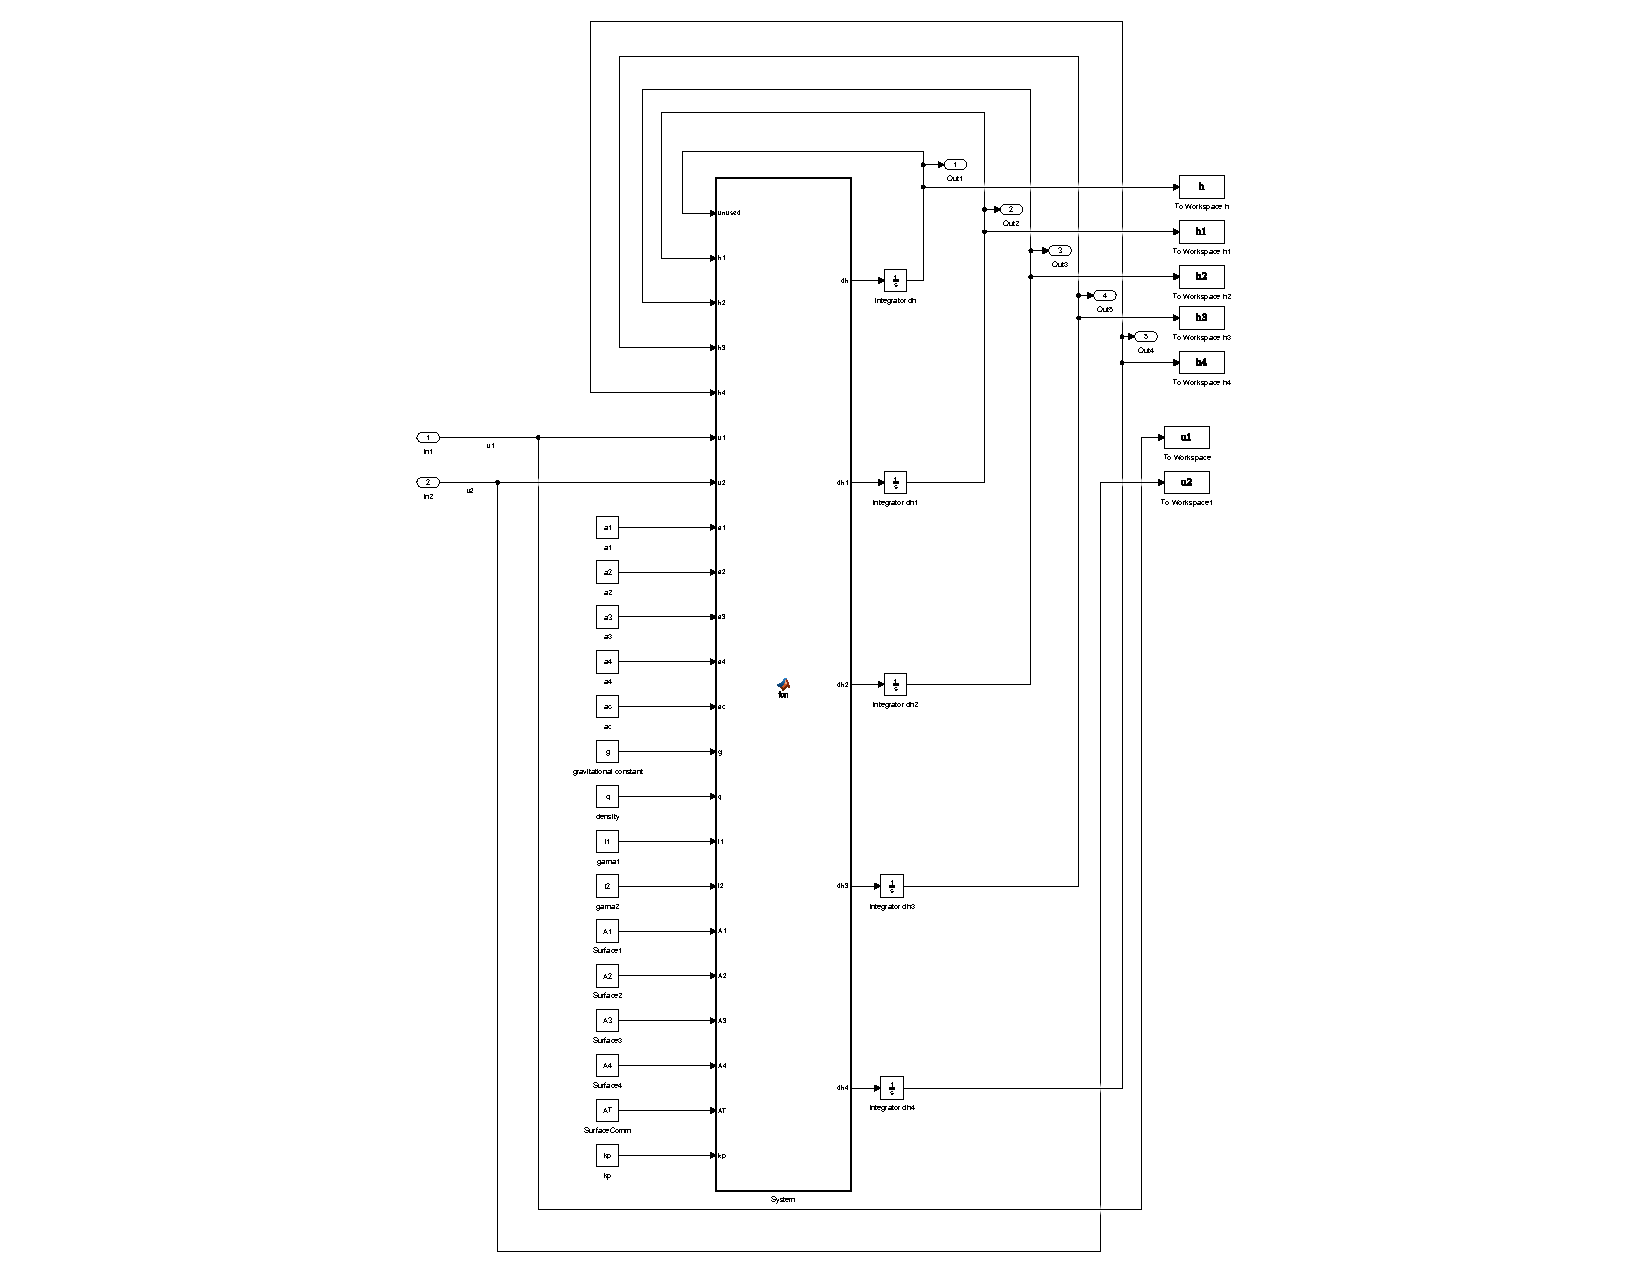
\includepdf[pages=-,pagecommand={},width=\textwidth]{system_schema.pdf}

% Consideram filtrul FIR de ordinul I:
% \begin{center}
% $\displaystyle H( z) \ =\ 1-cz^{-1} ,\ c\ =re^{j\theta } ,\ \theta \in [ 0,\ \pi ]$
% \end{center}

% \subparagraph {Pentru:\ $\displaystyle \theta \ =\ \pi /3$}

\myparagraph {Subpunctul a}

\begin{figure} [H]
	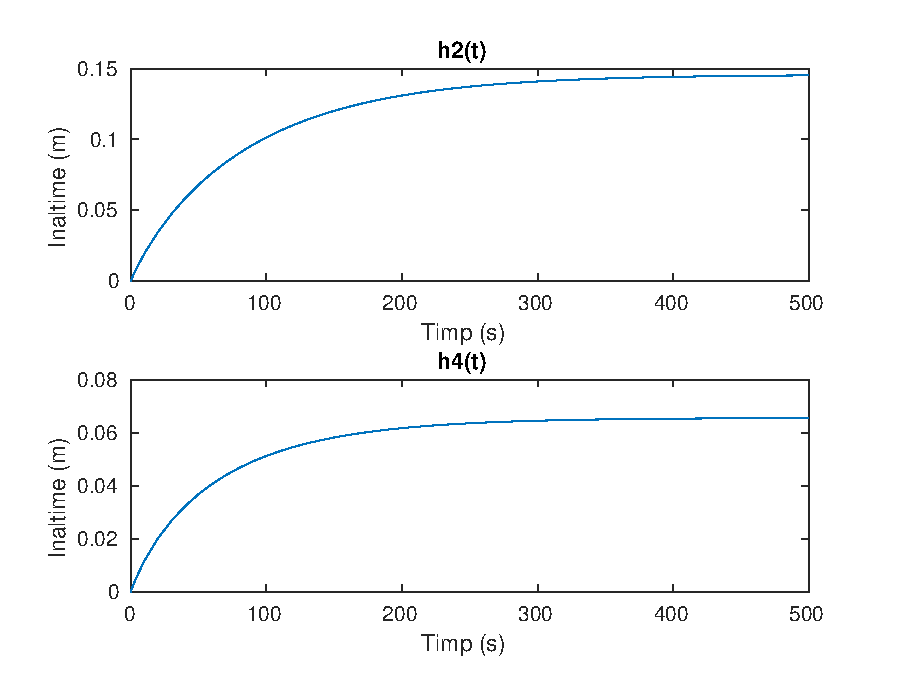
\includegraphics[width=1\textwidth]{a_2.eps}
	\caption{Evolutia iesirilor y2 si y4}
\end{figure}

\begin{figure} [H]
	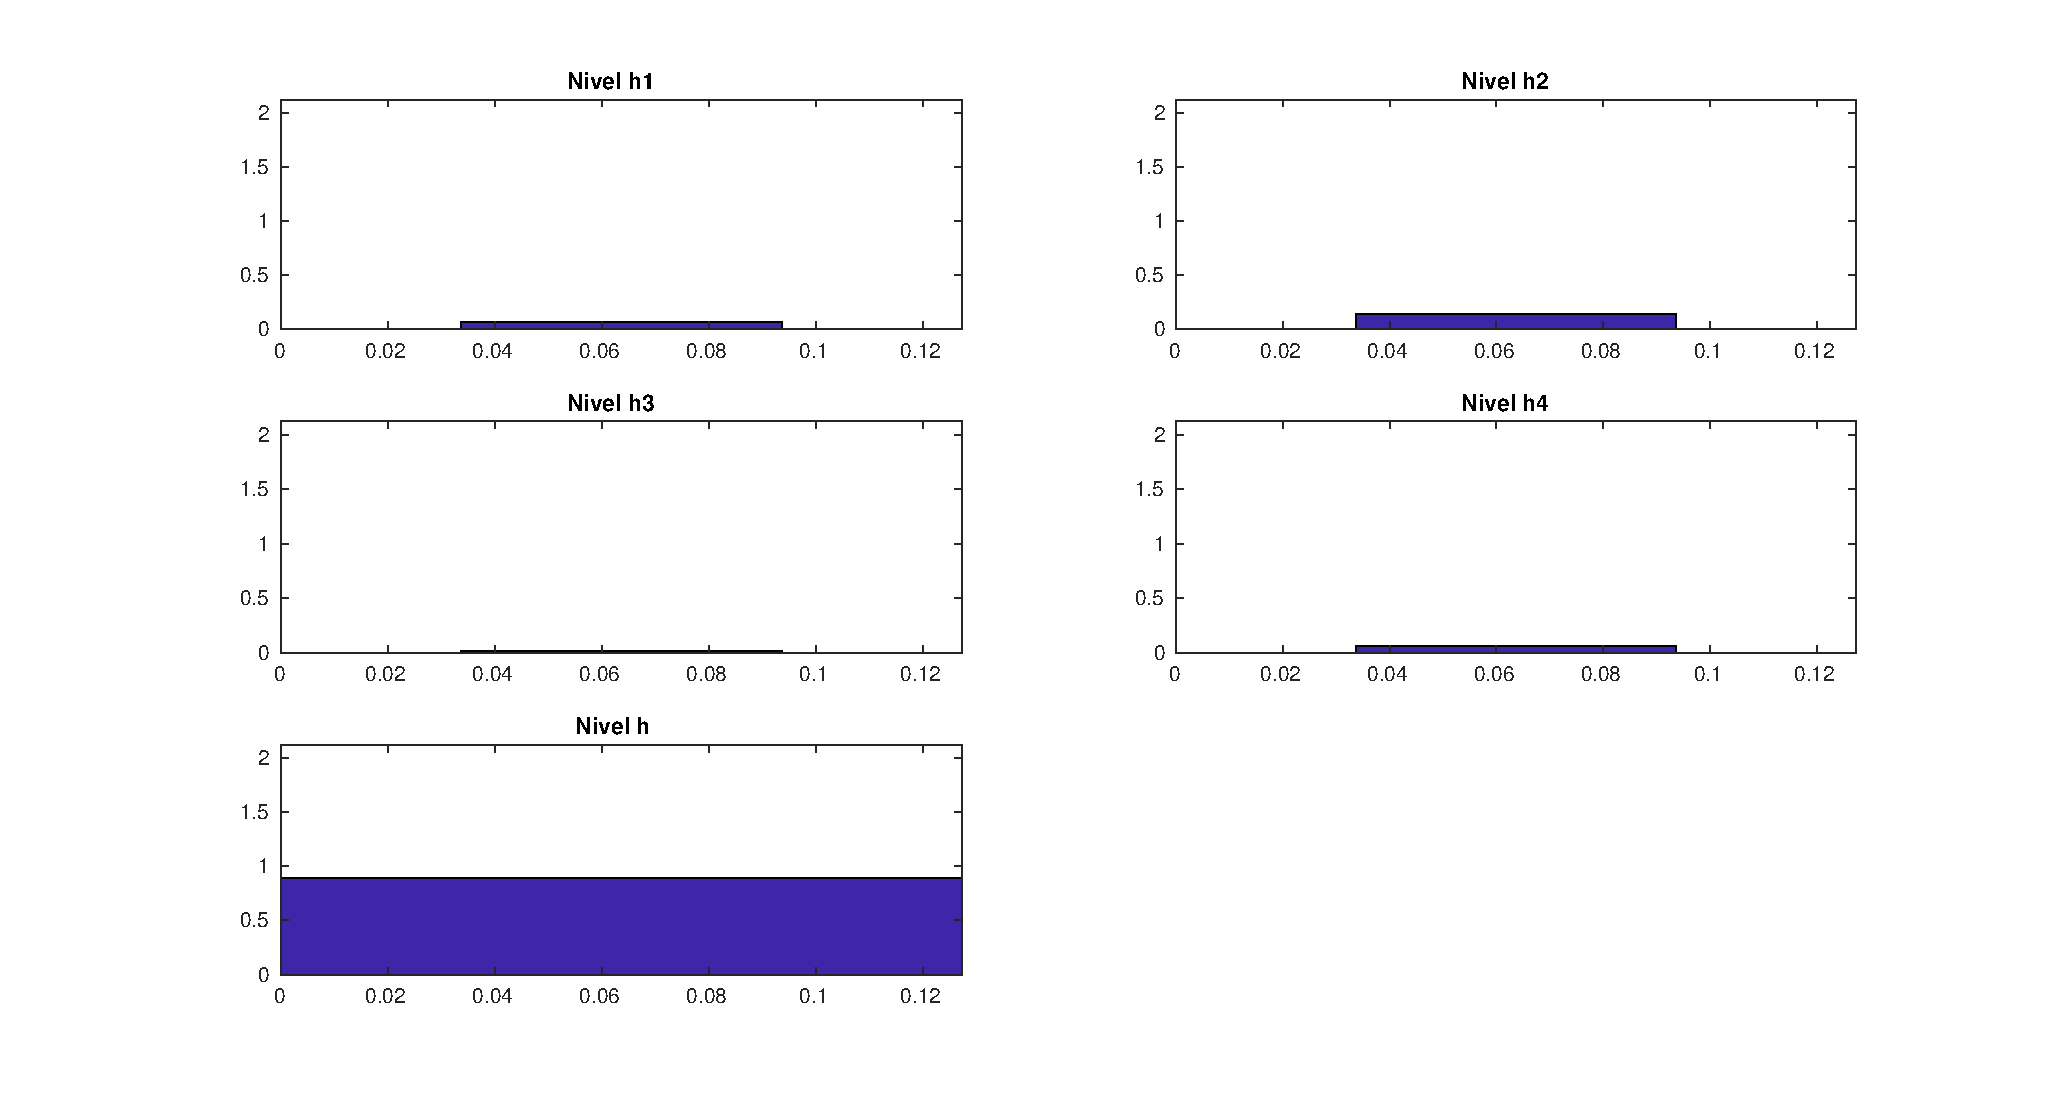
\includegraphics[width=1\textwidth]{a_1.eps}
	\caption{Exemplu animate levels}
\end{figure}

\myparagraph {Subpunctul b}
Pentru a varia conditiile initiale am creat vectorii \textit{arr\_cih, arr\_cih1, arr\_cih2, arr\_cih3, arr\_cih4} in fisierul \textit{load\_workspace\_b.m}, iar pentru a rula mai multe simulari se pot adauga dupa nevoie valori noi acestora.

\begin{figure} [H]
	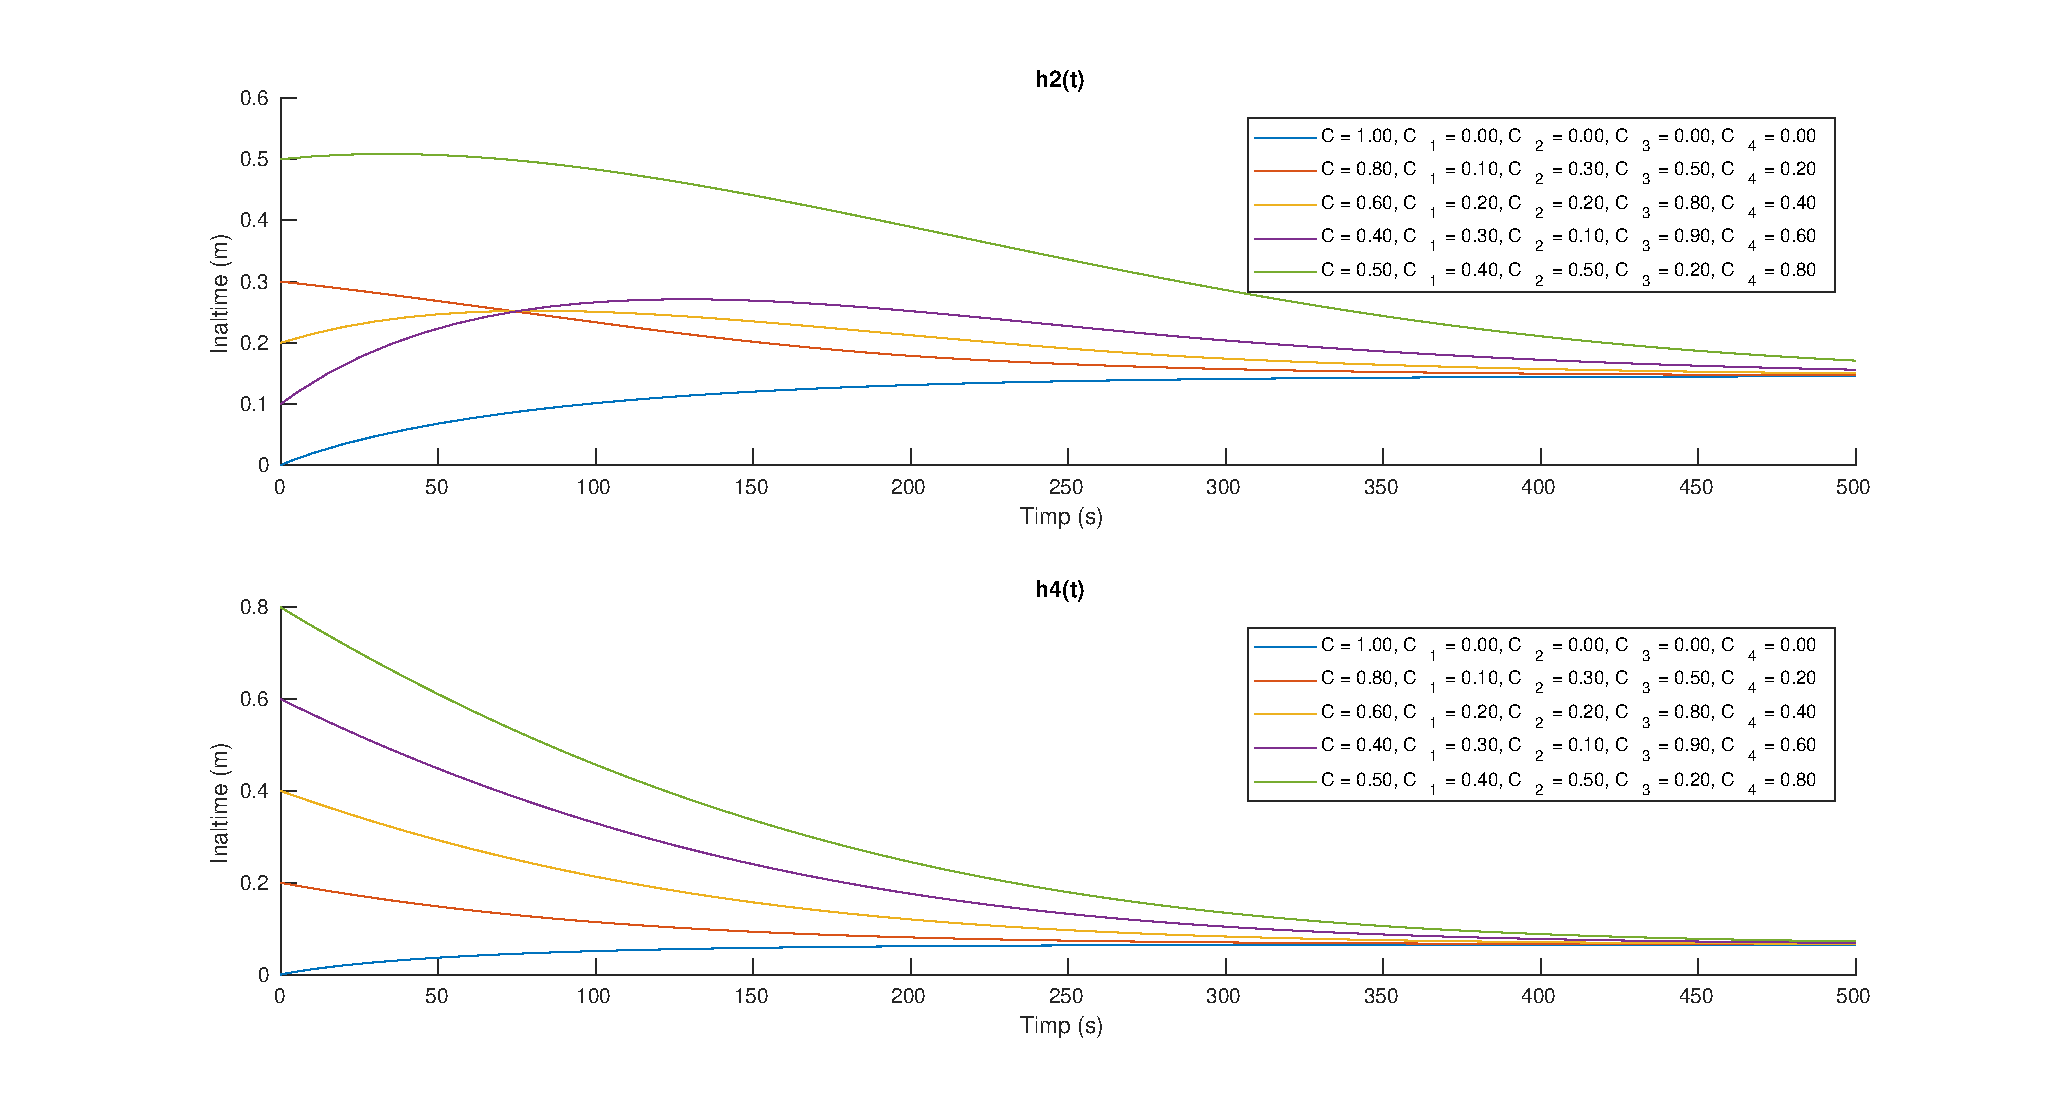
\includegraphics[width=1\textwidth]{b_1.eps}
	\caption{Evolutia iesirilor y2 si y4}
\end{figure}

\noindent{Se observa ca indiferent de volumul initial de lichid din rezervoare, iesirile sistemului se vor stabiliza in jurul aceluias punct.}

\pagebreak
\myparagraph {Subpunctul c}
Folosing functia \textit{stepinfo(h2.Data, h2.Time)} aflam informatii despre raspunsul sistemului si putem extrage timpul de stabilizare.

\begin{figure} [H]
	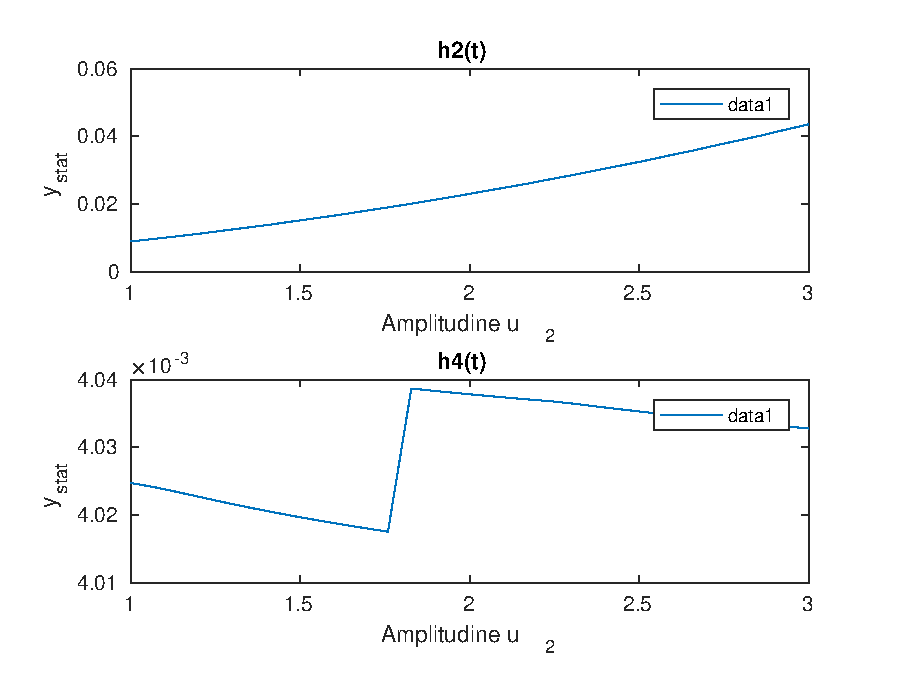
\includegraphics[width=1\textwidth]{c_1.eps}
	\caption{Evolutia iesirilor y2 si y4 in functie de valorile constantelor de integrare}
\end{figure}

\begin{figure} [H]
	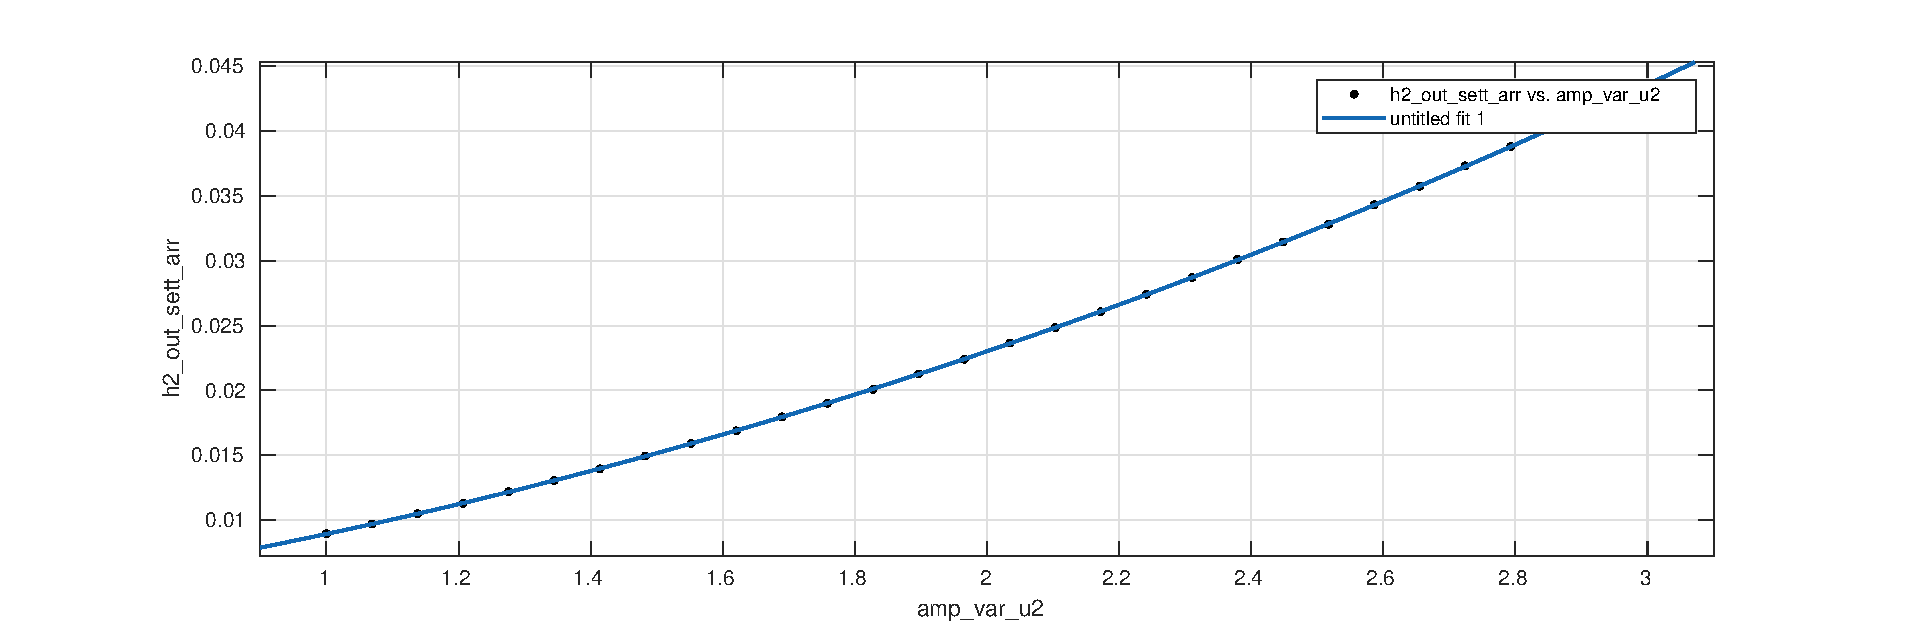
\includegraphics[width=1\textwidth]{c_2_1.eps}
	\caption{Stabilizare h2 in functie de amplitudinea intrarii}
\end{figure}

\pagebreak
\noindent{Cea mai buna aproximare se obtine cu polinomul de gradul 2:}

\begin{equation*}
f( x) \ =\ p1*x^{2} +p2*x+p3,\ \begin{cases}
		p1\ =\ 0.003242 & \\
		p2\ =\ 0.004348 & \\
		p3\ =\ 0.001353 & 
	\end{cases}
\end{equation*}


\begin{figure} [H]
	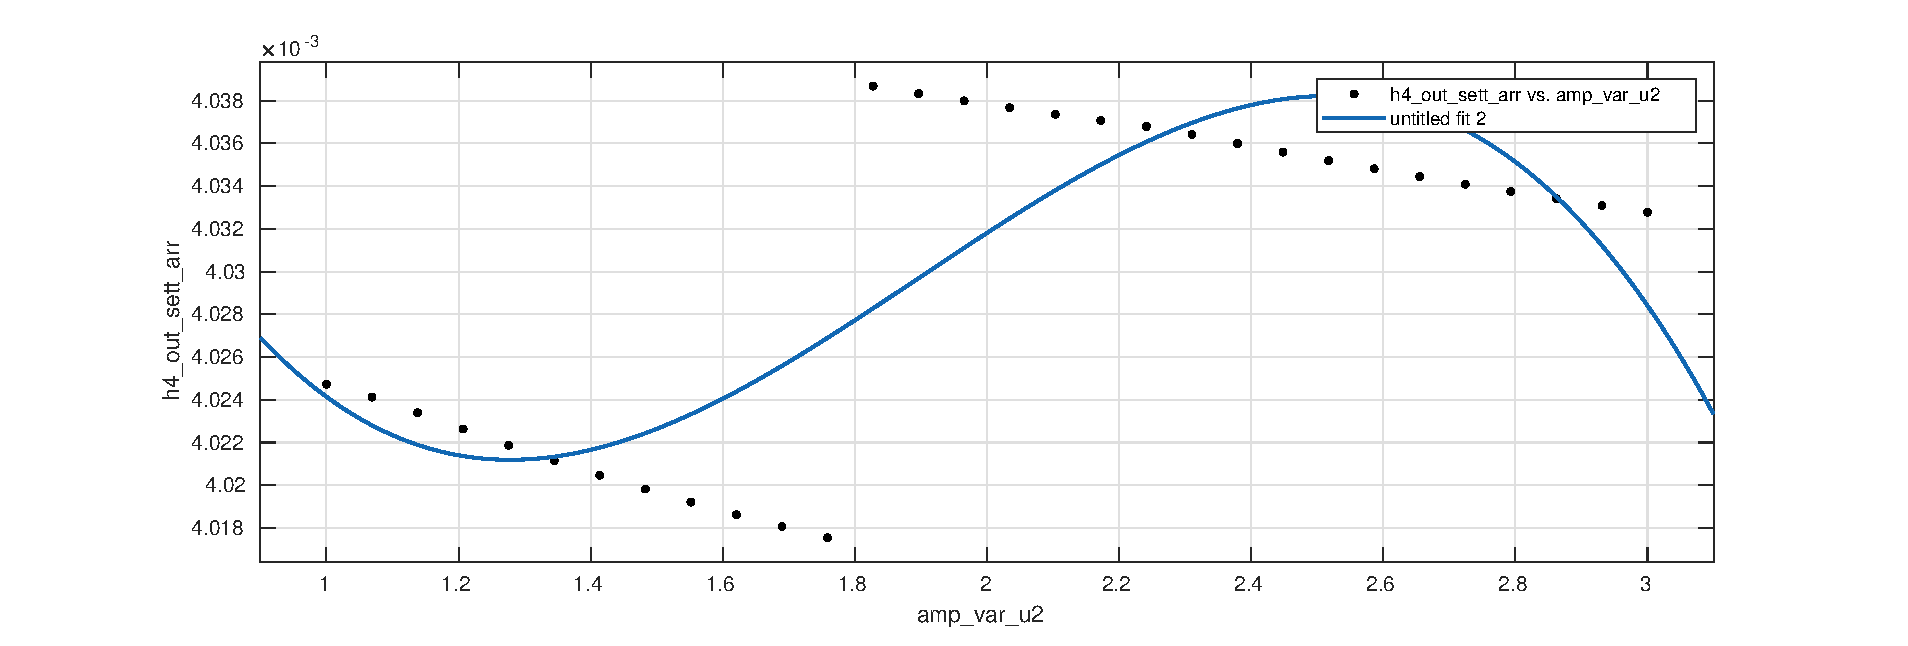
\includegraphics[width=1\textwidth]{c_2_2.eps}
	\caption{Stabilizare h4 in functie de amplitudinea intrarii}
\end{figure}

\begin{equation*}
f( x) \ =\ p1*x^{3} +p2*x^{2} +p3*x+p4,\ \begin{cases}
p1\ =\ -1.791e-05 & \\
p2\ =\ 0.000101 & \\
p3\ =\ -0.000172 & \\
p4\ =\ 0.004113 & 
\end{cases}
\end{equation*}

\myparagraph {Subpunctul d}

\noindent{Dupa trecerea timpului de stabilizare am aplicat urmatorul algoritm pentru a afla aproximarea liniara, unde j este primul index dupa stabilizare:}
\begin{minted}{matlab}
[A, B, C, D] = linmod(model_name, ...
	[h.Data(j) h1.Data(j) h2.Data(j) h3.Data(j) h4.Data(j)], ...
	[u1_data(j) u2_data(j)]);

linsys = ss(A, B, C, D);
out = lsim(linsys, [u1_data; u2_data]', u1_time');

ti = linspace(0, 300, 300);

nonlinear_out_2 = interp1(h2.Time, h2.Data, ti);
linear_out_2 = interp1(u2_time, out(:, 3), ti);
\end{minted}

\begin{figure} [H]
	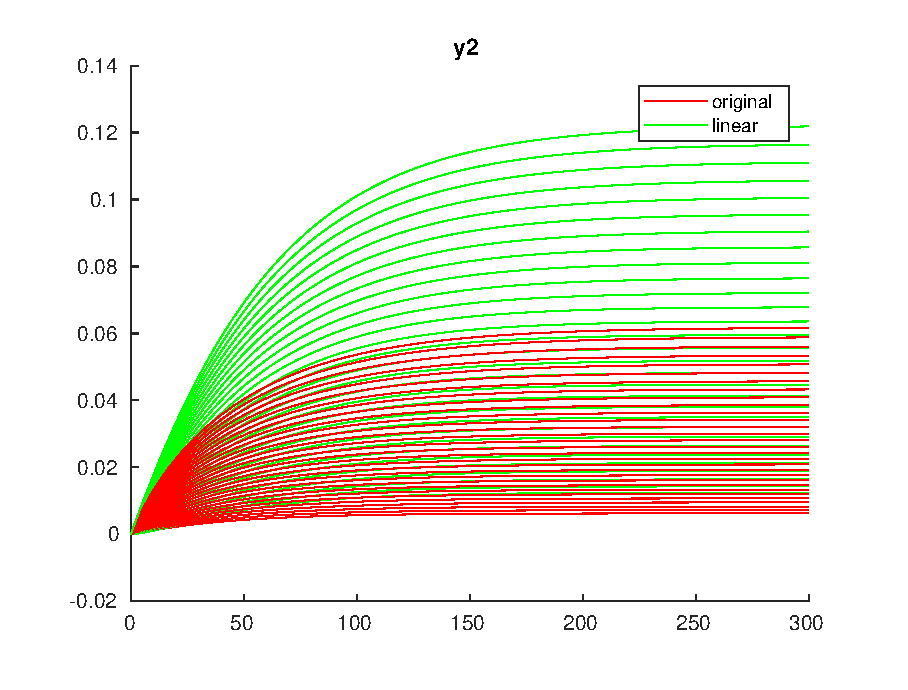
\includegraphics[width=1\textwidth]{d_1.eps}
	\caption{Evolutia iesirii h2 vs aproximarea sa liniara}
\end{figure}

\begin{figure} [H]
	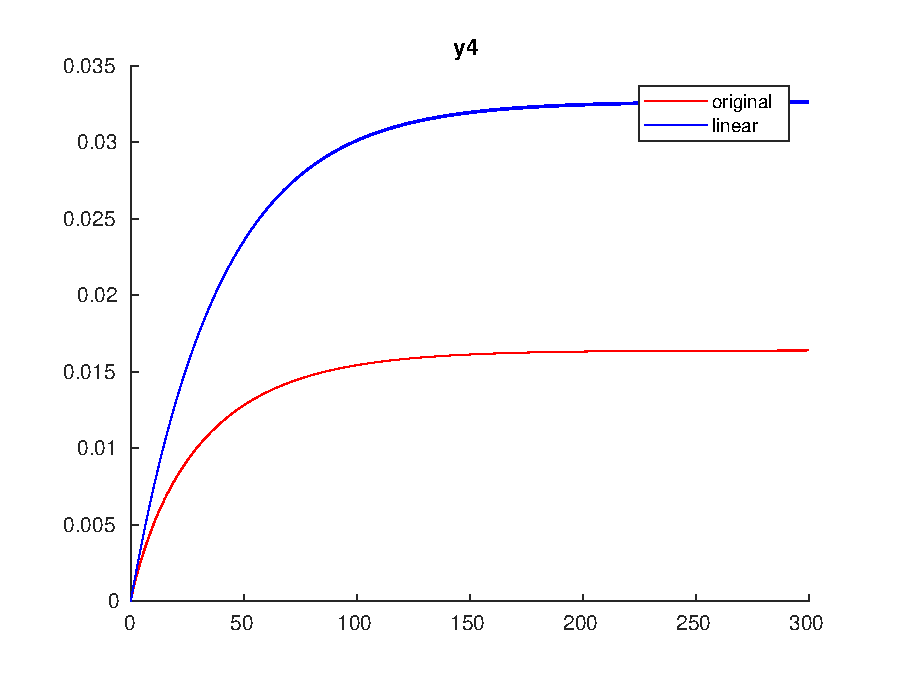
\includegraphics[width=1\textwidth]{d_2.eps}
	\caption{Evolutia iesirii h4 vs aproximarea sa liniara}
\end{figure}

\myparagraph {Subpunctul e}
Pentru a putea calcula eroarea cu ajutorul formulei din enunt, am interpolat vectorii iesirilor simiularii si aproximarii sale liniare astfel, stocand rezultatul in variabilele \textit{error\_sys\_2(i, j)} si \textit{error\_sys\_4(i, j)}:

\begin{minted}{matlab}
linsys = ss(A, B, C, D);

for j=1:loop_len
	amp_u2 = amp_var_u2(j);

	u2_time = 0:time_step:time_count;
	u2_data = ones(1, length(u2_time)) * amp_u2;
	u2 = [u2_time' u2_data'];

	res = sim(model_name,'StartTime','0','StopTime','300','FixedStep','0.02');

	h  = res.h;
	h1 = res.h1;
	h2 = res.h2;
	h3 = res.h3;
	h4 = res.h4;

	out = lsim(linsys, [u1_data; u2_data]', u1_time');

	ti = linspace(1, 300, 300);

	nonlinear_out_2 = interp1(h2.Time, h2.Data, ti);
	linear_out_2 = interp1(u2_time, out(:, 3), ti);

	nonlinear_out_4 = interp1(h4.Time, h4.Data, ti);
	linear_out_4 = interp1(u2_time, out(:, 5), ti);

	error_sys_2(i, j) = ...
		norm((linear_out_2 - nonlinear_out_2) ./ nonlinear_out_2);
	
	error_sys_4(i, j) = ...
		norm((linear_out_4 - nonlinear_out_4) ./ nonlinear_out_4);
end
\end{minted}

\begin{figure} [H]
	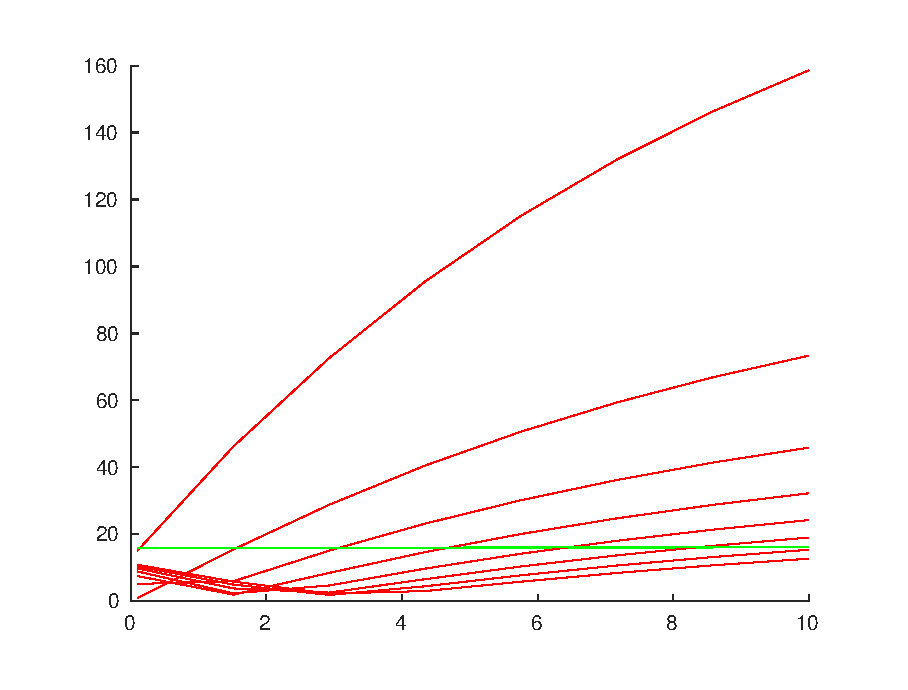
\includegraphics[width=1\textwidth]{e_1.eps}
	\caption{Graficele erorilor in functie de intrari}
\end{figure}

\pagebreak
\myparagraph {Subpunctul f}
Cautam eroarea minima in vectorul calculat la subpunctul anterior, cat si indexul la care aceasta apare eroare:

\begin{minted}{matlab}
[err_min, err_idx] = min(error_sys_2(i, :));
fprintf("Eroare min la j: %d => u2 = %d\n", err_idx, amp_var_u2(err_idx));
j_queue(i) = err_idx;
\end{minted}

\myparagraph {Subpunctul g}
Calculam raspunsul partial ``pe intervale'':

\begin{minted}{matlab}
out_1 = [];
out_2 = [];
last_i = 1;
last_x = [cih cih1 cih2 cih3 cih4];
for it=1:length(j_queue)
	j = j_queue(it);
	t = time_at(j);
	current_u1_data = [];
	current_u2_data = [];
	current_time = [];

	amp_u2 = amp_var_u2(j);
	u2_time = 0:time_step:time_count;
	u2_data = ones(1, length(u2_time)) * amp_u2;
	u2 = [u2_time' u2_data'];

	while (u1_time(last_i) < t)
		current_time(end + 1) = u1_time(last_i);
		current_u1_data(end + 1) = u1_data(last_i);
		current_u2_data(end + 1) = u2_data(last_i);
		last_i = last_i + 1;
	end
	[out, last_t, last_x] = lsim(linsys{j}, [current_u1_data; current_u2_data]', ...
		current_time', last_x(end, :));

	out_1 = [out_1; out(:, 3)];
	out_2 = [out_2; out(:, 5)];
end
\end{minted}

\myparagraph {Subpunctul h}
Pentru a afla eroare de urmarire, calculam integrala:

\begin{minted}{matlab}
fun = @(i) abs(nonlinear_out_2(int32(i)) - partial_linear_out_2(int32(i)));
err_2 = integral(fun, ti(1), ti(end));

fun = @(i) abs(nonlinear_out_4(int32(i)) - partial_linear_out_4(int32(i)));
err_4 = integral(fun, ti(1), ti(end))

fprintf("Erorare de urmarire y2 = %f\n", err_2);
fprintf("Erorare de urmarire y4 = %f\n", err_4);
\end{minted}

\myparagraph {Grafice f, g, h}

\begin{figure} [H]
	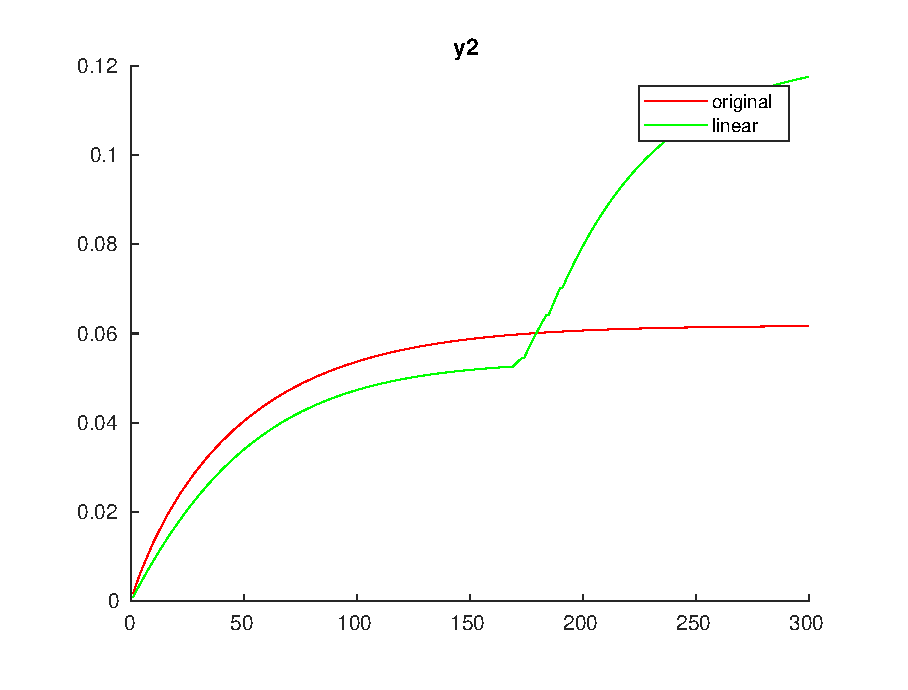
\includegraphics[width=1\textwidth]{fgh_1.eps}
	\caption{Evolutia iesirii h2 vs aproximarea sa liniara pe bucati}
\end{figure}

\begin{figure} [H]
	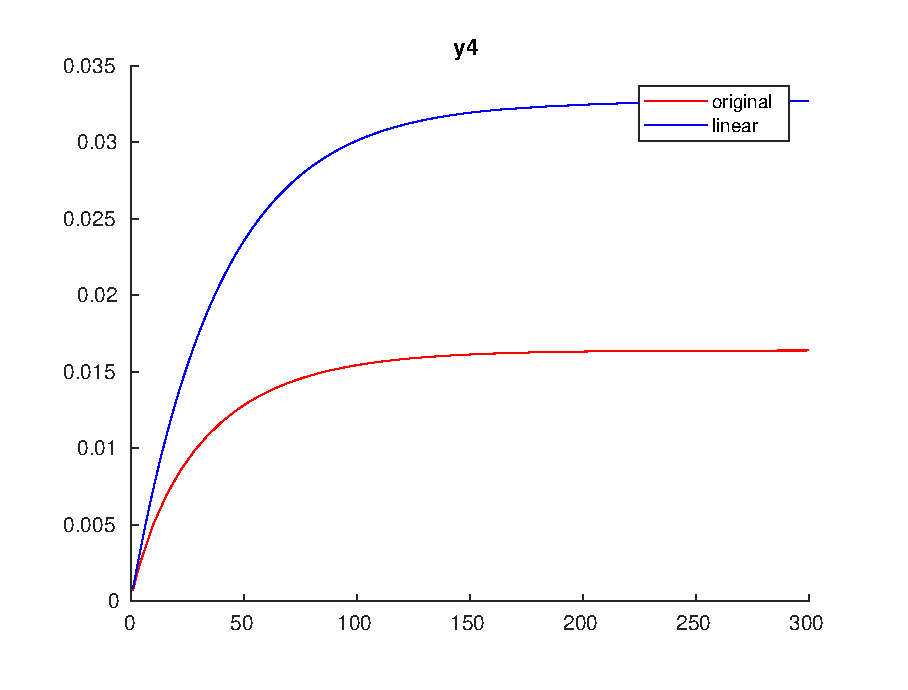
\includegraphics[width=1\textwidth]{fgh_2.eps}
	\caption{Evolutia iesirii h4 vs aproximarea sa liniara pe bucati}
\end{figure}

% 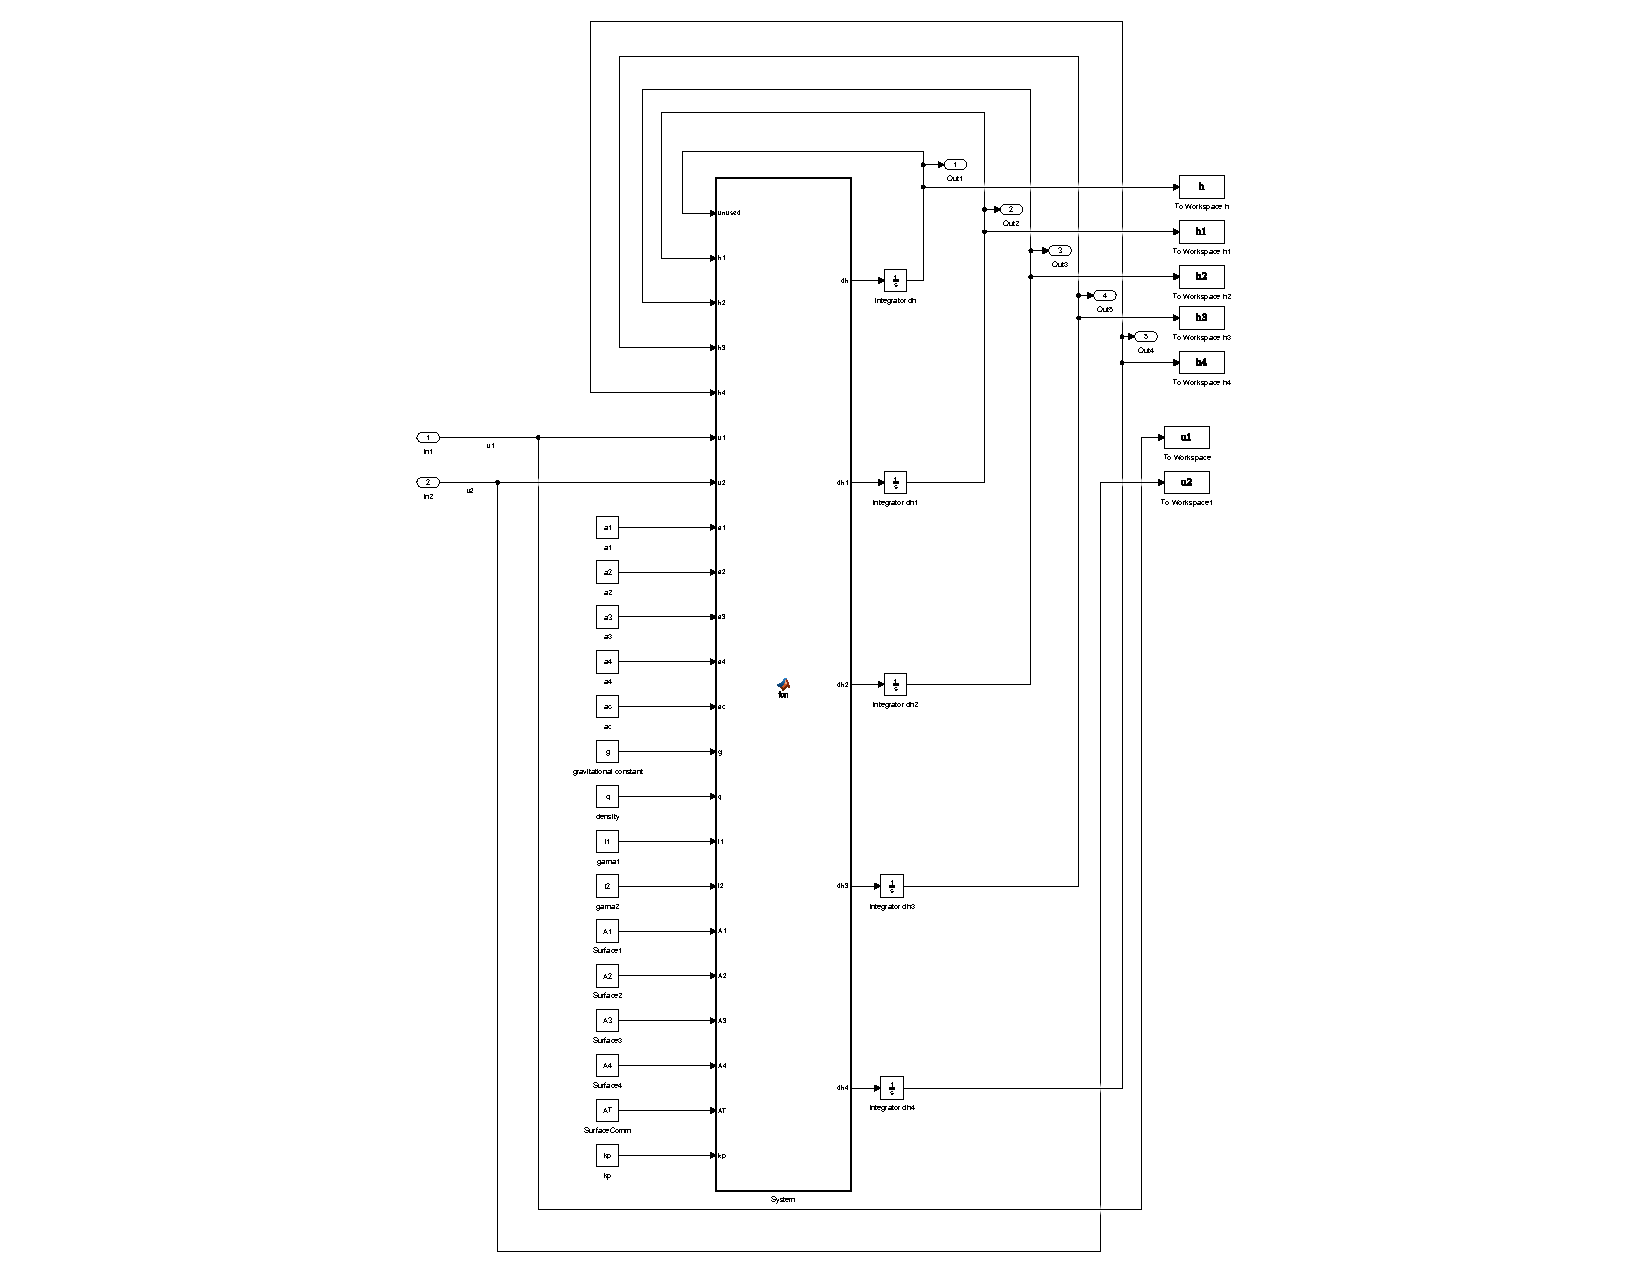
\includepdf[pages={1},lastpage={1}]{system_schema.pdf}
\pagebreak
\myparagraph {Model Simulink}
Cod functie:
\begin{minted}{matlab}
function [dh, dh1, dh2, dh3, dh4] = fcn(~, h1, h2, h3, h4,...
		u1, u2, a1, a2, a3, a4, ac, g, q, l1, l2, A1, A2, A3, A4, AT, kp)

    dh1 = 1/A1*(-a1*sqrt(2*g*h1) - ac*sign(q*g*h1 - q*g*h2)*sqrt(2*g*abs(h1 - h2)) + ...
    	a3*sqrt(2*g*h3) + l1*kp*u1);
    dh2 = 1/A2*(-a2*sqrt(2*g*h2) - ac*sign(q*g*h1 - q*g*h2)*sqrt(2*g*abs(h1 - h2)) + ...
    	a4*sqrt(2*g*h4) + l2*kp*u2);
    dh3 = 1/A3*(-a3*sqrt(2*g*h3) + (1 - l2)*kp*u2);
    dh4 = 1/A4*(-a4*sqrt(2*g*h4) + (1 - l1)*kp*u1);
    dh = 1/AT*(a1*sqrt(2*g*h1) + a2*sqrt(2*g*h2) - kp*u1 - kp*u2);
end
\end{minted}

\begin{figure} [H]
	\hspace*{-.25\textwidth}
	\includegraphics[width=1.5\textwidth]{system_schema.eps}
	\caption{Diagrama bloc Simulink}
\end{figure}

\end{document}